\chapter{拉普拉斯变换与连续时间系统}
\label{chap:laplace-transform}

\section{用微分方程描述因果 LTI 系统}
\label{sec:ct-differential-equation}

第四章从单位冲激响应 $h(t)$ 出发，把系统输出写成卷积积分。这条路径要求先求出 $h(t)$，而电路和力学系统中的元件关系往往直接给出另一类等式：输入、输出及其各阶导数之间的关系。本节把这类方程讲清楚，包括它为什么不能单独确定一个系统、补上什么条件才对应因果 LTI 系统，以及怎样一步步算出响应。后面几节引入拉普拉斯变换后，同样的响应会有更省力的算法，但时域解法仍是判断适用条件的基础。

\subsection{微分方程给的是隐式关系}

先看电阻与电容串联的电路。以电容电压 $y(t)$ 为输出、电压源 $x(t)$ 为输入，基尔霍夫定律与元件特性给出
\begin{equation}
  \frac{\dd y(t)}{\dd t}+ay(t)=bx(t),
  \label{eq:ct-first-order-generic}
\end{equation}
其中 $a=1/(RC)$，$b$ 由电源接法确定。同样的形式也出现在力学系统中：取车辆速度 $y(t)$、驱动力 $x(t)$，摩擦力使方程呈这个形状。

\cref{eq:ct-first-order-generic} 是\red{隐式（implicit）描述}：它约束输入与输出之间的关系，却没有把 $y(t)$ 写成 $x(t)$ 的显式表达式。要得到显式表达式必须解方程，而解方程还需要方程以外的信息。

\begin{intuition}[为什么一个方程不够]
  同一个电路，接上同样的电源，电容上原有的电压不同，之后的电压波形就不同。方程只描述电压怎样变化，不描述从哪里开始变。速度、电流、电荷都有惯性，方程给出变化的规律，起始状态必须另外交代。
\end{intuition}

\begin{example}[同一方程的三种结果]
  对\cref{eq:ct-first-order-generic} 取 $a=1$、$b=1$，输入 $x(t)=1$（$t>0$）。方程的解一般写成
  \[
    y(t)=1+A\e^{-t},\qquad t>0,
  \]
  其中 $A$ 完全由起始状态决定：
  \[
    y(0)=0\Rightarrow y(t)=1-\e^{-t},
    \quad
    y(0)=1\Rightarrow y(t)=1,
    \quad
    y(0)=2\Rightarrow y(t)=1+\e^{-t}.
  \]
  三条曲线满足同一个微分方程，却是三个不同的输入输出关系。\red{微分方程本身不构成一个确定的系统}。
\end{example}

\subsection{初始静止：因果 LTI 对辅助条件的要求}

要选定一个系统，必须补上辅助条件（auxiliary conditions）。初始储能不为零时，即使输入为零，输出也会因为储能释放而存在一段响应，整个系统也不再是线性的。讨论由微分方程描述的因果 LTI 系统时，统一采用初始静止（initial rest）条件。

\begin{definition}[初始静止]
  \label{def:ct-initial-rest}
  若输入满足 $x(t)=0$（$t\leq t_0$），则输出也满足 $y(t)=0$（$t\leq t_0$）。
\end{definition}

它\red{不等于让零时刻取值取零}，而是把归零的时刻跟着输入走。输入从 $t_0$ 起才非零，就以 $t_0$ 作为起算点。物理含义是：接入电源之前电路里没有任何储能；今天做实验和明天做实验，只差一个时间平移。

对 $N$ 阶方程，初始静止落在 $N$ 个初始条件上。一般的 $N$ 阶线性常系数微分方程（linear constant-coefficient differential equation）写作
\begin{equation}
  \sum_{k=0}^{N}a_k\frac{\dd^k y(t)}{\dd t^k}
  =\sum_{k=0}^{M}b_k\frac{\dd^k x(t)}{\dd t^k},
  \label{eq:ct-lccde}
\end{equation}
输出的最高求导阶数 $N$ 称为方程的阶。若 $x(t)=0$（$t\leq t_0$），初始静止要求
\begin{equation}
  y(t_0)=\left.\frac{\dd y(t)}{\dd t}\right|_{t=t_0}
  =\cdots=\left.\frac{\dd^{N-1}y(t)}{\dd t^{N-1}}\right|_{t=t_0}=0.
  \label{eq:ct-initial-rest-conditions}
\end{equation}
在这组条件下，\cref{eq:ct-lccde} 描述的系统是\red{因果且线性时不变}的：输出只依赖输入当前与过去的取值，初始状态固定为零，输入叠加或平移时解按同样方式叠加或平移。

\begin{pitfall}[把零状态响应与全响应混为一谈]
  按初始静止解出的响应是零状态响应，即假设初始储能为零时的输出。题目若另外给出 $y(0^-)$、$y'(0^-)$ 之类的初始条件，总响应还要加上零输入响应，\red{不能直接写成 $Y(s)=H(s)X(s)$}。后续各节只讨论零状态响应；遇到带初始条件的题目，先拆成两项分别计算。
\end{pitfall}

\subsection{时域求解的一般形式}

初始静止下求解\cref{eq:ct-lccde}，解仍由两部分相加而成：
\[
  y(t)=y_{\mathrm h}(t)+y_{\mathrm p}(t).
\]
$y_{\mathrm h}(t)$ 是齐次解，即右端取零后方程
\[
  \sum_{k=0}^{N}a_k\frac{\dd^k y(t)}{\dd t^k}=0
\]
的通解，对应系统的自然响应；$y_{\mathrm p}(t)$ 是一个特解，形式通常与输入一致。方程的阶数决定齐次解中待定常数的个数。

手算按下面的顺序进行：

\begin{enumerate}
  \item 写出特征方程 $\sum_{k=0}^{N}a_ks^k=0$，由特征根写齐次解。单实根 $s$ 给出 $\e^{st}$；$r$ 重根给出 $t^{m}\e^{st}$（$m=0,\ldots,r-1$）；共轭复根 $s=\sigma\pm\iu\omega$ 给出 $\e^{\sigma t}\cos\omega t$ 与 $\e^{\sigma t}\sin\omega t$。
  \item 按输入形式设特解。输入为 $t^{m}$ 时设同次多项式，输入为 $\e^{st}$ 时设 $Y\e^{st}$ 并代回求 $Y$。\red{特解与齐次解中某项重合时须乘 $t$}，否则代回后左边为零，系数定不出来。
  \item 代入初始静止条件，定出齐次解中的待定常数。
  \item 回代验证。把解及其导数代入原方程，检查在 $t=0^+$ 附近是否成立。
\end{enumerate}

\begin{remark}[与时域卷积的关系]
  初始静止下求出的响应既是零状态响应，按第四章的结论它又等于 $x(t)\conv h(t)$。由\cref{eq:ct-lccde} 解出的 $h(t)$ 就是该系统的单位冲激响应；只要能解出 $h(t)$，任意输入都可由卷积得到，同一个系统的不同输入只需重复最后一步卷积。
\end{remark}

\section{一阶方程：指数输入与冲激响应}
\label{sec:ct-first-order-example}

\begin{workedexample}[一阶微分方程的零状态响应]
  \label{ex:ct-first-order-exponential}
  因果连续时间 LTI 系统满足
  \[
    \frac{\dd y(t)}{\dd t}+3y(t)=x(t),
  \]
  输入为 $x(t)=\e^{-2t}\stepfun(t)$。求零状态响应。
\end{workedexample}

\begin{solution}
  特征方程为 $s+3=0$，特征根 $s=-3$，齐次解
  \[
    y_{\mathrm h}(t)=A\e^{-3t}.
  \]
  输入在 $t>0$ 时为 $\e^{-2t}$，指数 $-2$ 不是特征根，故设特解 $y_{\mathrm p}(t)=Y\e^{-2t}$。代入原方程，
  \[
    -2Y\e^{-2t}+3Y\e^{-2t}=\e^{-2t}
    \quad\Longrightarrow\quad Y=1,
  \]
  于是 $y_{\mathrm p}(t)=\e^{-2t}$，通解为
  \[
    y(t)=A\e^{-3t}+\e^{-2t},\qquad t>0.
  \]
  输入在 $t<0$ 为零，由初始静止得 $y(0)=0$，代入解得 $A=-1$。合并两段，
  \[
    \boxed{y(t)=\bigl(\e^{-2t}-\e^{-3t}\bigr)\stepfun(t)}.
  \]
  它在 $t=0$ 处为零，而
  \[
    \left.\frac{\dd y}{\dd t}\right|_{t=0^+}=1,
  \]
  与方程在 $0^+$ 处给出的 $y'(0^+)=x(0^+)-3y(0^+)=1$ 一致。响应在 $t=\ln\frac32$ 处达到峰值，随后按 $\e^{-2t}$ 衰减，见\cref{fig:ex-ct-first-order-answer}。
  \begin{figure}[H]
    \centering
    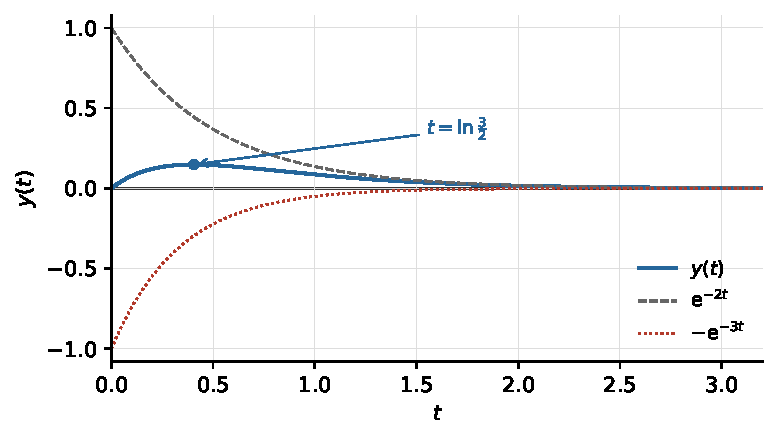
\includegraphics[width=0.78\textwidth]{09-laplace-transform/examples/first-order-answer.pdf}
    \caption{例题 \ref{ex:ct-first-order-exponential} 的零状态响应。曲线由 $\e^{-2t}$ 与 $-\e^{-3t}$ 两项叠加而成，峰值位置由 $y'(t)=0$ 定出。}
    \label{fig:ex-ct-first-order-answer}
  \end{figure}
\end{solution}

\begin{technique}
  一阶方程解出 $y_{\mathrm h}$ 后，先检查特解形式是否与齐次项重合：输入指数与特征根相同时要乘 $t$。定常数只用初始静止给出的一个条件，代入前先写清起算点处的取值为零。输入在 $t=0$ 才接入时，该条件退化为 $y(0)=0$。
\end{technique}

\section{二阶方程与阶跃输入}
\label{sec:ct-second-order-example}

\begin{workedexample}[二阶微分方程对阶跃输入的响应]
  \label{ex:ct-second-order-step}
  因果连续时间 LTI 系统满足
  \[
    \frac{\dd^2y(t)}{\dd t^2}+3\frac{\dd y(t)}{\dd t}+2y(t)=x(t),
  \]
  输入为 $x(t)=\stepfun(t)$。求零状态响应，并说明它与冲激响应的关系。
\end{workedexample}

\begin{solution}
  特征方程
  \[
    s^2+3s+2=(s+1)(s+2)=0
  \]
  给出两个互异实根 $s=-1$、$s=-2$，齐次解为
  \[
    y_{\mathrm h}(t)=A\e^{-t}+B\e^{-2t}.
  \]
  输入在 $t>0$ 时为常数 $1$，设特解 $y_{\mathrm p}(t)=C$。代入原方程，$0+0+2C=1$，得 $C=\frac12$，常数特解对应稳态值。

  输入在 $t<0$ 为零，由初始静止得 $y(0)=0$ 与 $y'(0)=0$。把通解
  \[
    y(t)=A\e^{-t}+B\e^{-2t}+\frac12
  \]
  及其导数在 $t=0^+$ 处取值，得到两个方程
  \[
    A+B+\frac12=0,\qquad -A-2B=0.
  \]
  由第二式得 $A=-2B$，代入第一式得 $-B+\frac12=0$，故
  \[
    B=\frac12,\qquad A=-1.
  \]
  因此
  \[
    \boxed{y(t)=\Bigl(\frac12-\e^{-t}+\frac12\e^{-2t}\Bigr)\stepfun(t)}.
  \]
  两个初始条件都用上了，这也是\red{阶数决定条件个数}的体现。结果中随时间衰减的两项由特征根决定，常数项由输入决定。响应从零开始，起始斜率为零，单调上升到 $1/2$，见\cref{fig:ex-ct-second-order-answer}。
  \begin{figure}[H]
    \centering
    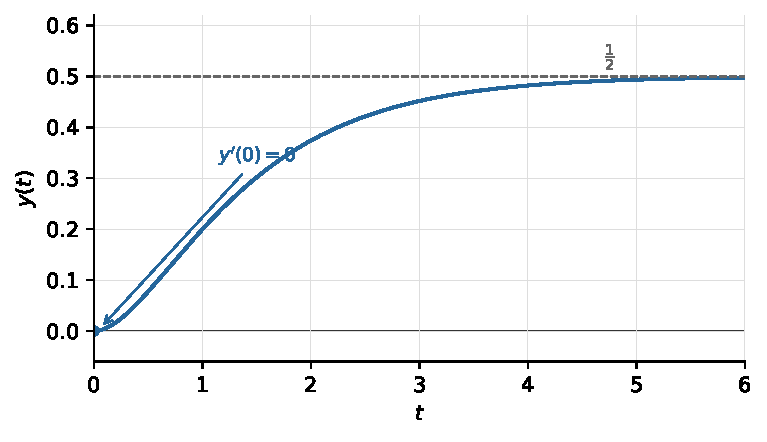
\includegraphics[width=0.78\textwidth]{09-laplace-transform/examples/second-order-answer.pdf}
    \caption{例题 \ref{ex:ct-second-order-step} 的零状态响应。曲线在 $t=0$ 处函数值与导数都为零，水平虚线为稳态值 $\frac12$。}
    \label{fig:ex-ct-second-order-answer}
  \end{figure}

  该系统的冲激响应可对 $y$ 求导得到。$y$ 在 $t=0$ 连续，求导只需处理 $t>0$ 的部分再加阶跃因子：
  \[
    h(t)=y'(t)=\bigl(\e^{-t}-\e^{-2t}\bigr)\stepfun(t).
  \]
  冲激响应与阶跃响应满足第四章的求导关系，可用来独立核对。
\end{solution}

\begin{technique}
  二阶方程要两个初始条件，初始静止时就是 $y(0)=0$ 与 $y'(0)=0$，一个都不能少。特解取常数说明输入含直流分量，稳态值等于特解。解完阶跃响应可对 $t$ 求导得到冲激响应，两者互相印证，能查出齐次解系数中的错误。
\end{technique}

\section{阶跃响应的比例关系与单位冲激响应}
\label{sec:ct-input-derivative}

\begin{workedexample}[阶跃响应的比例关系与冲激响应]
  \label{ex:ct-input-derivative}
  因果连续时间 LTI 系统满足
  \[
    \frac{\dd y(t)}{\dd t}+2y(t)=b\stepfun(t),
  \]
  其中 $b$ 为非零常数。求零状态响应；说明 $b=1$ 与 $b=4$ 两条曲线的关系；再求系统的单位冲激响应。
\end{workedexample}

\begin{solution}
  特征根为 $s=-2$，齐次解 $A\e^{-2t}$。输入为常数 $b$，特解取常数 $C$，代入得 $2C=b$，即 $C=b/2$。通解
  \[
    y(t)=A\e^{-2t}+\frac b2.
  \]
  由初始静止 $y(0)=0$ 得 $A=-b/2$，故
  \[
    \boxed{y(t)=\frac b2\bigl(1-\e^{-2t}\bigr)\stepfun(t)}.
  \]
  响应单调上升，稳态值为 $b/2$，形状只由特征根 $\e^{-2t}$ 决定。$b$ 出现在每一项的系数里，因此 $b=4$ 时的波形\red{逐点取值为四倍}，见\cref{fig:ex-ct-input-derivative}。两条曲线都没有有限时刻的峰值，取值随时间单调趋于稳态。
  \begin{figure}[H]
    \centering
    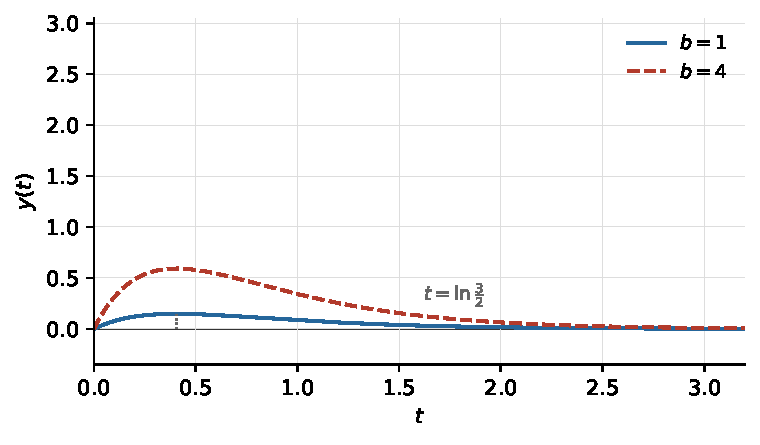
\includegraphics[width=0.78\textwidth]{09-laplace-transform/examples/impulse-input-rc.pdf}
    \caption{例题 \ref{ex:ct-input-derivative} 中阶跃响应的比例关系：右端系数由 $b=1$ 增至 $4$，波形形状不变，各时刻取值乘以 $4$。}
    \label{fig:ex-ct-input-derivative}
  \end{figure}

  求单位冲激响应时令 $x(t)=\impulse(t)$。齐次解形式不变，设
  \[
    h(t)=K\e^{-2t}\stepfun(t).
  \]
  把方程两端从 $0^-$ 积分到 $0^+$：右端
  \[
    \int_{0^-}^{0^+}\impulse(t)\dd t=1,
  \]
  左端第一项给出跳变 $h(0^+)-h(0^-)=K$，第二项的积分在区间长度趋于零时为零。于是 $K=1$，
  \[
    \boxed{h(t)=\e^{-2t}\stepfun(t)}.
  \]
  它绝对可积，系统 BIBO 稳定且符合因果判据 $h(t)=0$（$t<0$）。
\end{solution}

\begin{technique}
  右端系数 $b$ 只改变响应幅度，不改变特征根定出的时间常数。求直流增益时令所有导数项为零，得 $y_{\mathrm{ss}}=b/a_0$，可用来核对特解。求一阶系统的单位冲激响应不必重复待定系数法：设 $h(t)=K\e^{st}\stepfun(t)$，把方程在零时刻附近积分一次，跳变条件直接给出 $K$。
\end{technique}

\section{由积分器构成的方框图}
\label{sec:ct-block-diagram}

\cref{eq:ct-lccde} 还能用基本运算单元画成方框图，这对理解系统结构和用计算机仿真都有用。连续时间的一阶方程为
\[
  \frac{\dd y(t)}{\dd t}+ay(t)=bx(t).
\]
把它解出最高阶导数，
\[
  \frac{\dd y(t)}{\dd t}=bx(t)-ay(t),
\]
两端从 $-\infty$ 积到 $t$。初始静止下 $y(-\infty)=0$，积分与求导相消，得到
\begin{equation}
  y(t)=\int_{-\infty}^{t}\bigl[bx(\tau)-ay(\tau)\bigr]\dd\tau.
  \label{eq:ct-integrator-form}
\end{equation}
\cref{eq:ct-integrator-form} 说明系统只需加法器、数乘器与积分器三种单元：把 $y(t)$ 经数乘 $-a$ 后与 $bx(t)$ 相加，再积分一次即得 $y(t)$；积分结果又送回输入端的加法器，构成反馈。

\begin{remark}[为什么用积分器而不是微分器]
  直接由原方程解出 $y(t)$ 也能画图，但式中含 $\dd y/\dd t$，要用微分器实现。微分器对噪声极为敏感，输入上一点高频扰动会被放大成很大的导数，实际电路和仿真都不采用这种接法。改用积分器后，结构对噪声是平滑的，这也是一阶方程在变换域里更适合按 $H(s)$ 的分母因式来讨论的原因。
\end{remark}

方框图中的积分器同时承担记忆作用，它保存的积分值就是系统的状态。初始静止对应\red{积分器的初值为零}。差分方程的方框图用单位延时器代替积分器，两种结构在这一点上完全对应，下一章会具体写出。

\begin{remark}[与变换域解法的衔接]
  初始静止下把方程两端作拉普拉斯变换，求导变成乘 $s$，微分方程化为关于 $s$ 的代数方程。本节三个例题的答案都能用这一路线重算：分母 $(s+3)$、$(s+1)(s+2)$ 与部分分式一一对应，系数由初始静止条件确定。高阶方程用变换域求解的代数步骤少得多，这是后续各节展开变换方法的主要动因。
\end{remark}
